\documentclass{beamer}
\usepackage{hyperref}
\usepackage[T1]{fontenc}
\usepackage{tikz}
\newcommand\Background{%
\begin{tikzpicture}[remember picture,overlay]
\node[inner sep=0pt,outer sep=0pt,opacity=0.5]
  at (current page.center){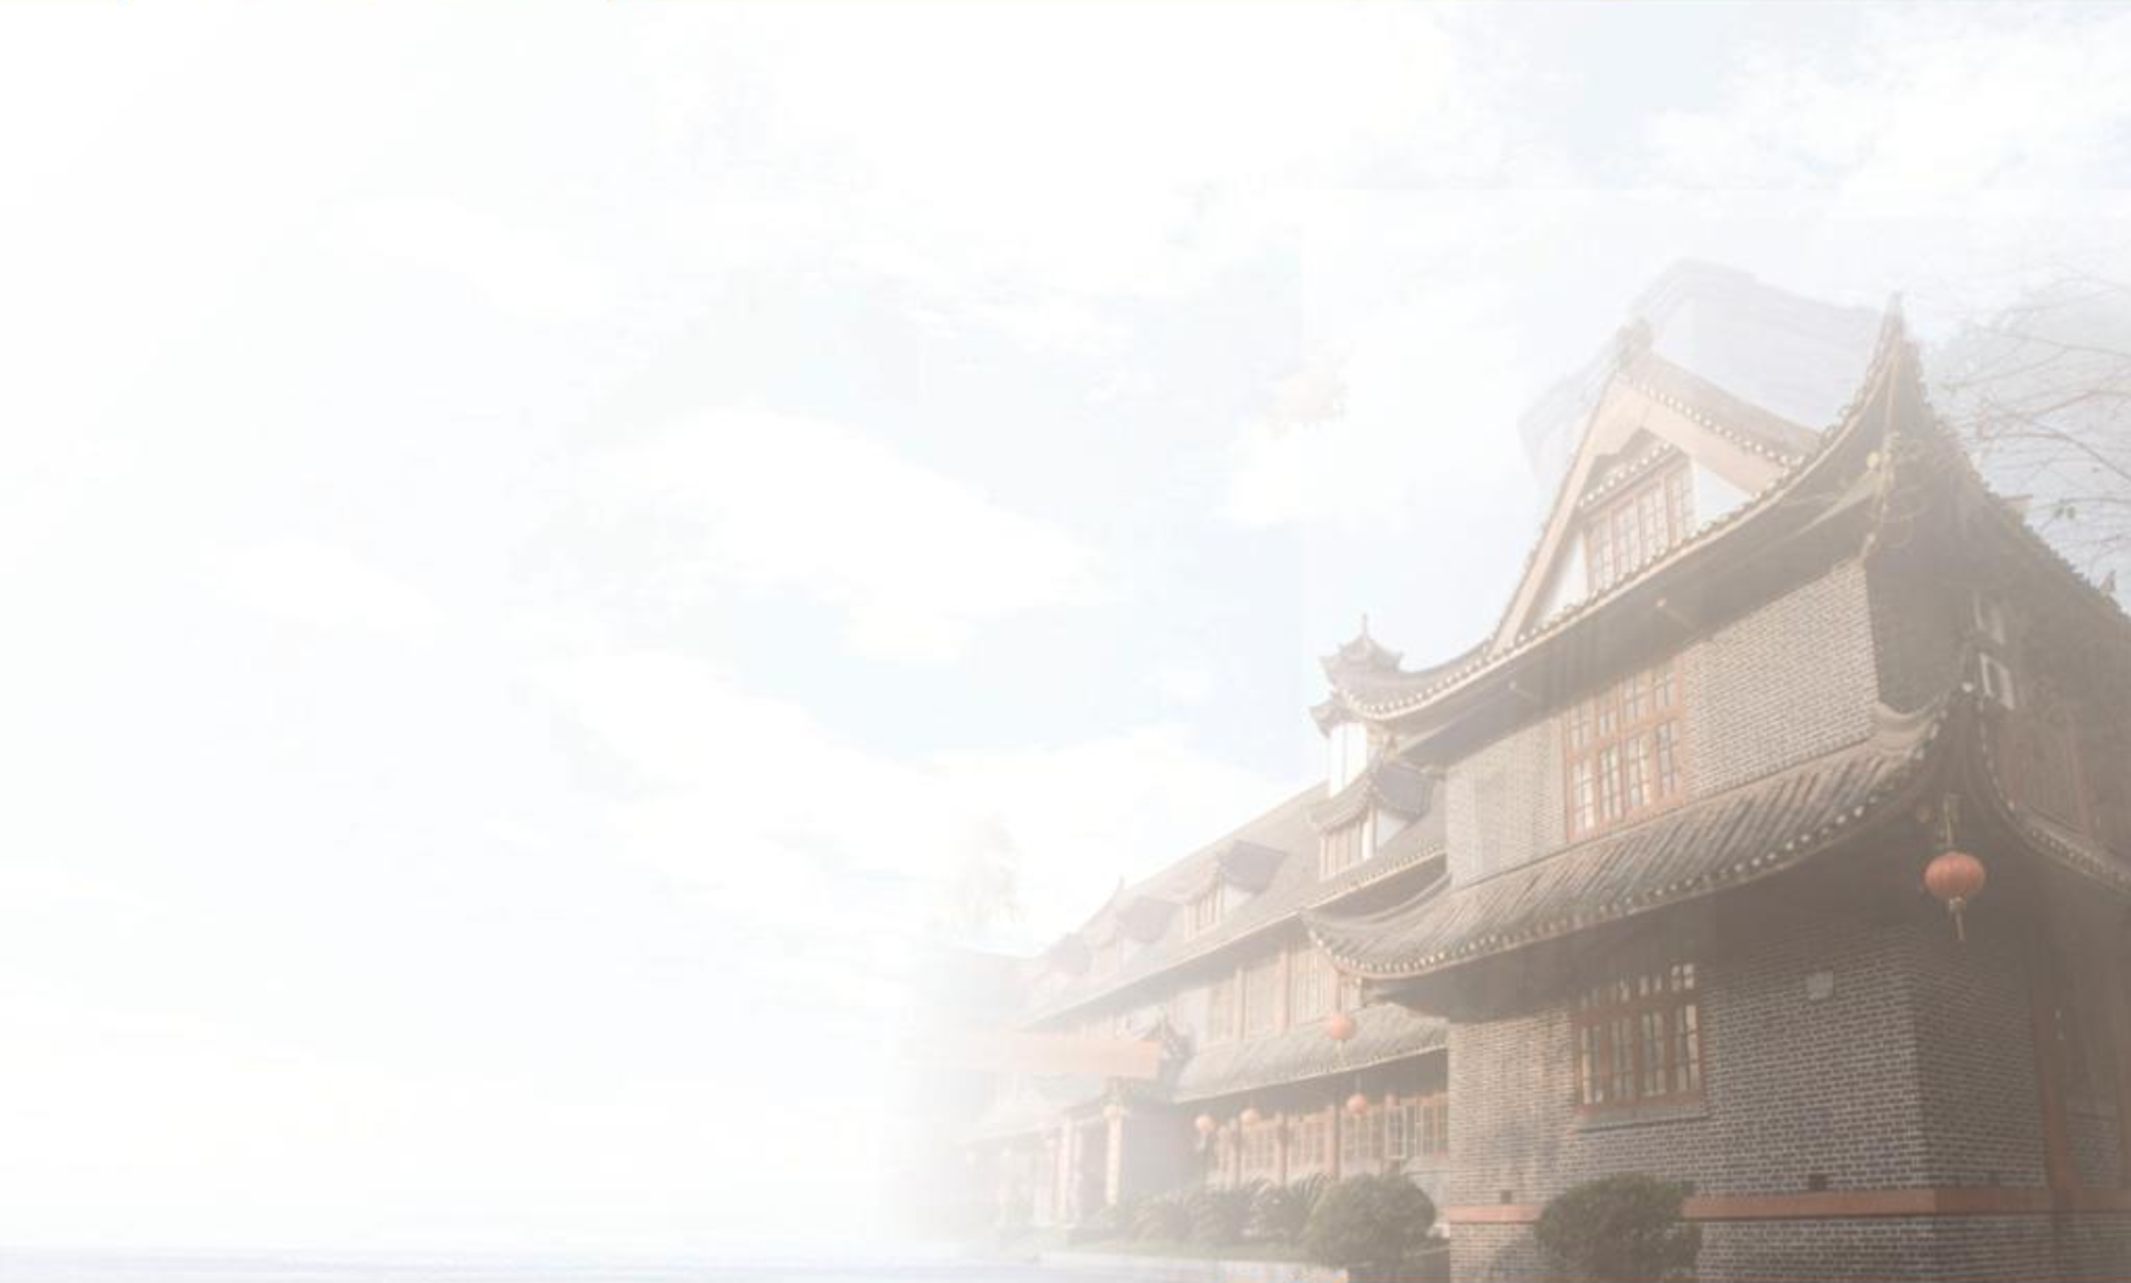
\includegraphics[width=1\paperwidth,height=1\paperheight]{fig/background.pdf}};
\end{tikzpicture}%
}
% other packages
\usepackage{latexsym,amsmath,xcolor,multicol,booktabs,calligra}
\usepackage{graphicx,pstricks,listings,stackengine}
\usepackage{cqu}

% packages and settings for bibtex
\usepackage[backend=bibtex,sorting=none]{biblatex}
\addbibresource{ref.bib}

\usefonttheme{serif}
\setbeamerfont{footnote}{size=\tiny}   % footnote for bibtex

\setbeamertemplate{bibliography item}[text]   % reference list for bibtex
\defbibheading{reference}{\section*{Reference}}   % heading for bibtex

\author[Xincao Xu]{Xincao Xu\\{\small near@cqu.edu.cn}}
\title{Chongqing University (CQU) Beamer Theme}
\subtitle{Using \LaTeX\ to prepare slides}
\institute{College of Computer Science\\
  Chongqing University}
\date[2022] % (optional)
{Created on Jun 02, 2022}

% defs
\def\cmd#1{\texttt{\color{red}\footnotesize $\backslash$#1}}
\def\env#1{\texttt{\color{blue}\footnotesize #1}}
\definecolor{cqublue}{RGB}{2,82,159} % Standard Color-CQU Blue
\definecolor{deepred}{rgb}{0.6,0,0}
\definecolor{deepgreen}{rgb}{0,0.5,0}
\definecolor{halfgray}{gray}{0.55}

\lstset{
    basicstyle=\ttfamily\small,
    keywordstyle=\bfseries\color{cqublue},
    emphstyle=\ttfamily\color{deepred},    % Custom highlighting style
    stringstyle=\color{deepgreen},
    numbers=left,
    numberstyle=\small\color{halfgray},
    rulesepcolor=\color{red!20!green!20!blue!20},
    frame=shadowbox,
}

\begin{document}

\begin{frame}
\Background
    \titlepage
    \begin{figure}[htpb]
        \begin{center}
            
\includegraphics[width=0.15\linewidth]{fig/Chongqing_University_Logo.pdf}
        \end{center}
    \end{figure}
\end{frame}   
\begin{frame}
\tableofcontents[sectionstyle=show,subsectionstyle=show/shaded/hide,subsubsectionstyle=show/shaded/hide]
\end{frame}

\section{Introduction}
\begin{frame}
	\begin{itemize}
		\item This template is a secondary creation of \href{https://github.com/Trinkle23897/THU-Beamer-Theme}{\color{purple}{Trinkle23897/THU-Beamer-Theme}} \cite{origin}
		\item This template is released under Creative Commons Zero BY 1.0 license
		\item This template follows \href{http://xiaoban.cqu.edu.cn/info/1037/2031.htm}{\color{purple}{Visual Identity System (VIS) of Chongqing University}}
	\end{itemize}
\end{frame}

\begin{frame}{Beamer for slides}
	\begin{itemize}
		\item We assume you can use \LaTeX; if not, you can learn it from {\href{http://en.wikibooks.org/wiki/LaTeX/}{\color{purple}here}}
		\item Beamer is one of the most popular and powerful document classes for presentations in \LaTeX
		\item Beamer has also a detailed \href{http://www.ctan.org/tex-archive/macros/latex/contrib/beamer/doc/beameruserguide.pdf}{\color{purple}{user manual}}
		\item Here we will present only the most basic features to get you up to speed
	\end{itemize} 
\end{frame}

\begin{frame}{Beamer vs. PowerPoint}
	Compared to PowerPoint, using \LaTeX\ is better because:
	\begin{itemize}
		\item It is not What-You-See-Is-What-You-Get, but
		What-You-\emph{Mean}-Is-What-You-Get:\\
		you write the content, the computer does the typesetting
		\item Produces a \texttt{pdf}: no problems with fonts, formulas,
      program versions
		\item Easier to keep consistent style, fonts, highlighting, etc.
		\item Math typesetting in \TeX\ is the best:
			\begin{equation*}
				\mathrm{i}\,\hslash\frac{\partial}{\partial t} \Psi(\mathbf{r},t) =
				-\frac{\hslash^2}{2\,m}\nabla^2\Psi(\mathbf{r},t)
				+ V(\mathbf{r})\Psi(\mathbf{r},t)
			\end{equation*}
		\end{itemize}
\end{frame}

\section{Slide Template}


\begin{frame}
\frametitle{Edge Computing}
\begin{columns}

\column{0.5\textwidth}
\begin{figure}
\centering
  \includegraphics[width=2.2in]{fig/fig_1.eps}
  \caption{Offloading the computing resources from the cloud data center to the edge of the network\footnotemark}
\end{figure}
\column{0.5\textwidth}
Advantage of Edge Computing
\begin{itemize}
\setbeamertemplate{itemize items}{$\bullet$}
	\item Low-latency
	\item High reliability
\end{itemize}

\end{columns}
\footnotetext{https://innovationatwork.ieee.org/real-life-edge-computing-use-cases/}
\end{frame}


\section{Summary}

\begin{frame}{Good Luck!}
	\begin{itemize}
		\item The latest version of this template is available on \href{https://github.com/neardws/Chongqing-University-Beamer-Theme}{\color{purple}{GitHub}}
		\item If you have corrections or suggestions, send them to \href{mailto:near@cqu.edu.cn}{\color{purple}{me}}
	\end{itemize}
\end{frame}

\begin{frame}{Reference}
	\printbibliography[heading=reference]
\end{frame}

\begin{frame}
\Background
    \begin{center}
        {\Huge Q\&A}\\
       	\textit{Thank you!}\\
       	\textit{Your feedback will be highly appreciated!}
    \end{center}
\end{frame}

\end{document}